\documentclass{beamer}

\usepackage{tcolorbox}
\usepackage{comment}
\usepackage{hyperref}
\usepackage{amsthm}
\usepackage{tikz}
\usepackage{graphicx}
\usepackage{amsmath}
% \usepackage[polish]{babel}
% \usepackage{polski}

% THIS IS GDANSK UNIVERSITY OF TECHNLOGOGY (PG) PRESENTATION TEMPLATE
% Creator: Jan Cychnerski <jan.cychnerski@eti.pg.edu.pl>
% Copyleft 2019


% PG THEME OPTIONS

\usetheme{Boadilla}
\usecolortheme{default}
\usefonttheme{professionalfonts}

% colors

\definecolor{PGBlue}{RGB}{0,56,101}
\definecolor{PGRed}{RGB}{193,10,39}
\definecolor{PGSilver}{RGB}{200,200,200}
\definecolor{PGBlack}{RGB}{0,0,0}

% PGBlue
\setbeamercolor{frametitle}{fg=PGBlue}
\setbeamercolor{normal text}{fg=PGBlue}
\setbeamercolor{structure}{fg=PGBlue}
\setbeamercolor{item}{fg=PGBlue}

% PGRed
\setbeamercolor{alerted text}{fg=PGRed}
\setbeamercolor{item projected}{fg=PGRed}

% white
\setbeamercolor{title}{fg=white}
\setbeamercolor{titlelike}{fg=white}
\setbeamercolor{subtitle}{fg=white}

% enumerate and itemize styles

\setbeamertemplate{itemize item}{\bfseries\color{PGRed}\raise1pt\hbox{\donotcoloroutermaths$\bullet$}}
\setbeamertemplate{itemize subitem}{\color{PGRed}\raise0.5pt\hbox{--}}
\setbeamertemplate{itemize subsubitem}{\color{PGRed}\tiny\raise1.5pt\hbox{\donotcoloroutermaths$\bullet$}}

\setbeamertemplate{enumerate item}{\bfseries\color{PGRed}\insertenumlabel.}
\setbeamertemplate{enumerate subitem}{\color{PGRed}\insertsubenumlabel.}
\setbeamertemplate{enumerate subsubitem}{\color{PGRed}\insertsubsubenumlabel.}
\setbeamertemplate{enumerate mini template}{\insertenumlabel}


% disable navigation

\beamertemplatenavigationsymbolsempty

% additional commands

\newcommand*{\vcenteredhbox}[1]{\begingroup
\setbox0=\hbox{#1}\parbox{\wd0}{\box0}\endgroup}

\graphicspath{{pgbeamer/}}


\usepackage{iflang}
\IfLanguageName{polish}{
\newcommand{\pglogobig}{pg-logo-big-pl}
\newcommand{\pglogosmall}{pg-logo-small-pl}
}{
\newcommand{\pglogobig}{pg-logo-big-en}
\newcommand{\pglogosmall}{pg-logo-small-en}
}


% FRAME TITLE LOGO
\addtobeamertemplate{frametitle}{\vcenteredhbox{\includegraphics[height=8mm]{\pglogosmall}}\bfseries}{}


\newcommand{\pgtitleframe}{{
% PG TITLE PAGE

\setbeamercolor{background canvas}{bg=PGBlue}
\setbeamercolor{title}{fg=white}
\setbeamercolor*{date}{fg=white}
\setbeamercolor*{author}{fg=white}

\setbeamertemplate{footline}{}

\begin{frame}[noframenumbering]
\centering
\vspace{1cm}
\includegraphics[height=3cm]{\pglogobig}
\vspace{5mm}
\maketitle
\end{frame}
}}

\newcommand{\pglastframe}{{
% PG LAST PAGE

\setbeamercolor{background canvas}{bg=PGBlue}
\setbeamercolor{title}{fg=white}
\setbeamercolor*{date}{fg=white}
\setbeamercolor*{author}{fg=white}

\setbeamertemplate{footline}{}

\begin{frame}[noframenumbering]
\centering
\vspace{1cm}
\includegraphics[height=5cm]{\pglogobig}
\end{frame}
}}


\makeatletter
\newenvironment<>{proofs}[1][\proofname]{%
    \par
    \def\insertproofname{#1\@addpunct{.}}%
    \usebeamertemplate{proof begin}#2}
  {\usebeamertemplate{proof end}}
\makeatother

\title[Token Swapping and Its Variants]{M07 - Complexity of Token Swapping and Its Variants}
\author{184657 Wojciech Panfil}
\date{30.10.2024}

\setbeamercovered{transparent}

\begin{document}
\pgtitleframe

\begin{frame}{Agenda}
    \begin{itemize}
        \item Reconfiguration problems
        \item Ladder lottery
        \item Token swapping - definition
        \item Upper bound on the minimum swapping seq length
        \item Lower bound on the minimum swapping seq length
        \item Simple Exact Algorithm
        \item Variant: Colored Token Swapping
        \item Colored Token Swapping - paths
        \item Colored Token Swapping - stars
    \end{itemize}
\end{frame}

\begin{frame}{Reconfiguration problems}
    Changing one feasible solution to another through a series of incremental steps, with each step also being a feasible solution
    \begin{itemize}
        \item Start - initial configuration (state)
        \item Goal - reach target configuration
        \item Transition must occur in predefined steps, satisfying constraints of the problem
        \item Each step is a valid solution
        \item Optimization - criteria such as shortest path, minimal resource usage, time efficiency.
        \item Example: Rubik's cube
    \end{itemize}
\end{frame}

\begin{frame}{Ladder lottery - Amidakuji}
    \begin{itemize}
        \item One of the most popular lotteries (in particular in Japan)
        \item Used to e.g assign roles to children in a group
        \item Example: 4 children - 2 of which need to clean the classroom.
        \item Vertical lines - top labels are children, bottom are roles.
        \item Horizontal lines - transitions - junctions.
        \item Going from the top of the vertical line turn at every junction.
    \end{itemize}
\end{frame}

\begin{frame}{Ladder lottery - Amidakuji}
    \begin{itemize}
        \item Step 0 - Teacher creates a ladder
        \item Step A - Teacher decides which endings indicate cleaning the classroom - check sign.
        \item Step B - Teacher covers the ladder and asks children to put their name randomly at the top endings of vertical lines.
        \item Step C - The ladder is uncovered and the roles are assigned.
    \end{itemize}
    \begin{center}
        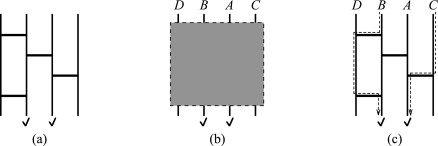
\includegraphics{../ladder.jpg}
    \end{center}
\end{frame}

\begin{frame}{Ladder lottery - Amidakuji}
    \begin{itemize}
        \item Vertical lines correspond to vertices in a graph.
        \item Horizontal lines correspond to edges in the graph.
        \item Going though the ladder is a sequence of swaps.
        \item The ladder transforms some initial permutation $f_0$ into a target one $f_t$
        \item There are many configurations of the ladder, which transform $f_0$ into $f_t$
        \item Problem: Which is the shortest one?
    \end{itemize}
    \begin{center}
        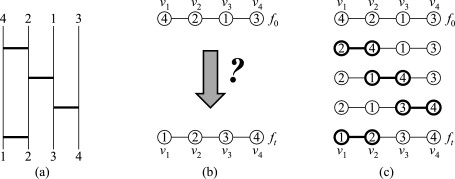
\includegraphics{../ladder_graph.jpg}
    \end{center}
\end{frame}

\begin{frame}{Ladder lottery - token swapping}
    \begin{itemize}
        \item Ladder lottery - an example of token swapping problem on a path.
        \item Each "vertex" is directly connected to its immediate neighbor.
        \item Swapping is restricted to adjacent vertical lines.
    \end{itemize}
\end{frame}

\begin{frame}{Token Swapping}
    \begin{itemize}
        \item \textbf{Definition:} Given a simple, connected graph \( G = (V, E) \) with a unique token on each vertex, the goal is to move all tokens to their designated target vertices using a sequence of adjacent swaps.
        \item \textbf{Objective:} Minimize the total number of swaps needed to reach the target configuration.
        \item \textbf{Key Elements:}
        \begin{itemize}
            \item \textit{Graph Structure:} Different complexities arise based on the graph type (e.g., path, tree, clique).
            \item \textit{Swapping Sequence (SS):} The sequence of moves that minimizes the swap count, denoted by $S$
            \item \textit{Applications:} Used in distributed systems, robotics, and even in games and puzzles.
        \end{itemize}
        \item \textbf{Parametrization:} By number of allowed swaps.
    \end{itemize}
\end{frame}

\begin{frame}{Token Swapping}
    \begin{tcolorbox}
        Suppose that the vertices in a graph $ G = (V, E)$ are assigned distinct labels $v_1, v_2, ..., v_n$. Let $ L = {1, 2, ..., n}$ be a set of $n$ labeled tokens.
        Then, a \textit{token placement} $f$ of $G$ is mapping $f : V$\textrightarrow$L$ such that $f(v_i) \neq f(v_j)$ holds for every two distinct vertices $v_i, v_j \in V$.
    \end{tcolorbox}
    \begin{tcolorbox}
        Image that tokens $f(v)$ are placed on the vertices $v$ of $G$. Since $f$ is a one-to-one correspondence, we can obtain its inverse mapping $f^{-1} : L$\textrightarrow$V$.
    \end{tcolorbox}
    \begin{itemize}
        \item $f_0$ denotes initial token placement
        \item $f_t$ denotes target token placement
        \item $OPT(f_0)$ denotes the optimal number of swaps needed to reach $f_t$ (shortest possible SS)
    \end{itemize}
\end{frame}

\begin{frame}{Token Swapping}
    \textbf{Complexity:}
    \begin{itemize}
        \item NP-hard as an optimization problem - finding the minimum number of swaps,
        \item NP-complete as a decision problem with a swap limit $k$ specified.
    \end{itemize}
    Note that this may vary for specific types of graphs such as path or cliques, being solvable in polynomial time.
\end{frame}

\begin{frame}{Adjacency of token placements}
    Two token placements $f$ and $f'$ of graph $G = (V, E)$ are adjacent if:
    \begin{itemize}
        \item Exactly one edge $(v_i, v_j) \in E(G)$ exists such that $f'(v_i) = f(v_j)$ and $f'(v_j) = f(v_i)$
        \item $f'(v_k) = f(v_k)$ for all vertices $v_k \in V \setminus {v_i, v_j}$
    \end{itemize}
    In other words, token placement $f'$ is obtained from $f$ by swapping the tokens on two vertices $v_i$ and $v_j$ such that $(v_i, v_j) \in E(G)$.
\end{frame}

\begin{frame}{Upper bound on minimum length of SS}
    \begin{tcolorbox}[title=Theorem 1: Upper Bound on minimum length of SS]
        For any initial token placement $f_0$ of a graph $G$, the optimal swap sequence length $OPT(f_0)$ satisfies:
        $OPT(f_0) = \mathcal{O}(n^2)$
    \end{tcolorbox}
    \vspace{0.5em}
    \begin{itemize}
        \item This implies that any instance of the \textit{Token Swapping} problem has a swapping sequence with a length bounded by a quadratic function of the number of vertices $n$.
        \item The quadratic bound provides an efficient estimate for complex swap sequences in arbitrary token placements.
    \end{itemize}
\end{frame}

\begin{frame}{Upper bound on minimum length of SS}
    \begin{proof}
    \begin{itemize}
        \item Let $T$ be any spanning tree of $G$.
        \item Choose an arbitraty leaf $v_i$ of $T$.
        \item Let $v_j$ be a vertex in $V$ such that $f_0(v_j) = i$.
        \item Moving the token $i$ from current position $v_j$ to $v_i$:
        \begin{itemize}
            \item Let $(w_1, w_2, ..., w_q)$ be a unique path in $T$ from $w_1 = v_j$ to $w_q = v_i$.
            \item Swap token on $w_k$ and $w_{k+1}$ for each $k = 1, 2, ..., q-1$ in this order.
            \item Finally, token placement $f$ of $G$ is obtained such that $f(v_i) = i$.
            \item Delete $v_i$ from $G$ and $T$ and repeat the process until $f_t$ is obtained.
        \end{itemize}
        \item Each token $i$ ($1 \leq i \leq n)$, can reach its target position $v_i$ via a swapping sub-sequence of length $\mathcal{O}(n)$.
        \item Having that, the swapping sequence $S$ between $f_0$ and $f_t$ satifies $len(S) = \mathcal{O}(n^2)$.
        \item Since $OPT(f_0) \leq len(S)$, we have $OPT(f_0) = \mathcal{O}(n^2)$
    \end{itemize}
    \end{proof}
\end{frame}

\begin{frame}{Lower bound on minimum length of SS}
    \begin{itemize}
        \item For a graph $G$ and two vertices $v, w \in V(G)$ we denote by ${sp}_G$ the number of edges in shortest path on $G$ between $v$ and $w$.
        \item Recall that $f^{-1}(i)$ denotes the vertex on which the token $i$ is placed in $f$.
        \item Furthermore, $f_t^{-1}(i)$ for all tokens $i$,$ 1 \leq n$ in the target token placement $f_t$.
        \item A potential function $p_G(f)$ is introduced as follows:
    \end{itemize}

    \begin{tcolorbox}[title=(1) Potential function $p_g(f)$]
        $p_G(f) = \sum_{1 \leq i \leq n}sp_G(f^{-1}(i), f_t^{-1}(i))$
    \end{tcolorbox}
    It indicates sum of shortest path length of all tokens from their position in $f$ to the target positions. In particular, $p_G(f_t) = 0$.
\end{frame}

\begin{frame}{Lower bound on minimum length of SS}
    \begin{tcolorbox}[title=Lemma 1: Lower bound on minimum length of SS]
        $OPT(f_0) \geq 0.5p_G(f_0)$ for any token placement $f_0$ of a graph $G$.
    \end{tcolorbox}
\end{frame}

\begin{frame}{Lower bound on minimum length of SS}
    \begin{proofs}
        Since $p_G(f_t) = 0$, it is sufficient to show that (2) $| p_G(f') - p_G(f) | \leq 2$ holds for any two adjacent token placements $f$ and $f'$ of $G$.
        \begin{itemize}
            \item Let $f$ and $f'$ be two adjacent token placements of $G$.
            \item There exists exactly one edge $(u, w)$ in $G$ such that $f'(u) = f(w)$ and $f'(w) = f(u)$.
            \item Let $i = f(u)$ and $j = f(w)$.
            \item Observe that $|sp_G(w, f_t^{-1}(i)) - sp_G(u, f_t^{-1}(i)) | \leq 1$ and $|sp_G(u, f_t^{-1}(j)) - sp_G(w, f_t^{-1}(j)) | \leq 1 $
        \end{itemize}
    \end{proofs}
\end{frame}

\begin{frame}{Lower bound on minimum length of SS}
    \begin{proof}
        \begin{itemize}
            \item Total change in the potential function can be denoted as
        \end{itemize}
        \begin{tcolorbox}[title=Total change in potential function due to swap]
            $|sp_G(w, f_t^{-1}(i)) - sp_G(u, f_t^{-1}(i))| + |sp_G(u, f_t^{-1}(j)) - sp_G(w, f_t^{-1}(j))| \leq 2$
        \end{tcolorbox}
        Since each swap decreases the potential function $p_G(f)$ by at most $2$, reducing $p_G(f_0)$ to $0$ will require at least $0.5p_G(f_0)$ swaps meaning
        \begin{tcolorbox}
            $OPT(f_0) \geq 0.5p_G(f_0)$ for any token placement $f_0$ of a graph $G$.
        \end{tcolorbox}
    \end{proof}
\end{frame}

\begin{frame}{Simple Exact Algorithm}
    The algorithm uses \textit{BFS} on a configuration graph to find the shortest sequence of swaps that transforms an initial token placement $f_0$ to a target
    token placement.
    \begin{enumerate}
        \item The configuration graph $G' = (V', E')$ represents all possible token placements on the vertices of the original graph $G$.
        \item Each node (vertex) $V'$ represents a unique token placement (permutation) on the graph $G$.
        \item Since each token placement is a unique arrangement of $n$ tokens, the number of nodes is $n!$ or $2^{\mathcal{O}(nlogn)}$
        \item Each edge $E'$ corresponds to a possible single swap between adjacent tokens. (It exists if one permutation can be obtained from another by a single swap of tokens between two adjacent vertices.)
    \end{enumerate}
\end{frame}

\begin{frame}{Simple Exact Algorithm}
    \begin{enumerate}
        \item For any token placement $A$, a adjacent token placement $B$ is reachable by a single swap between two adjacent vertices in $G$.
        \item Each configuration has at most $m =\mathcal{O}(n^{2})$ neighbors, since there are $\mathcal{O}(n^2)$ possible edges in a complete graph on $n$ vertices.
        \item Therefore, the total number of edges in the configuration graph is at most $0.5n!m$.
    \end{enumerate}
    \begin{tcolorbox}[title=Goal of the algorithm]
        Find the shortest sequence of swaps needed to transport the start permutation into the target one. This sequence corresponds to the shortest path between the start and target permutation
        in the configuration graph.
    \end{tcolorbox}
\end{frame}

\begin{frame}{Simple Exact Algorithm}
    \begin{enumerate}
        \item BFS is used to explore the configuration graph.
        \item It is ideal for this purpose as it finds the shortest path in an unweighed graph, which ensures the minimum number of swaps.
        \item Starting from initial permutation, BFS systematically explores all neighboring configurations (those that can be reached by a single swap)
        \item When it reaches the target configuration, it means the shortest sequence of swaps has been found.
    \end{enumerate}
    \textbf{Issue:} The configuration graph is large, with $n!$ nodes and up to $\mathcal{O}(n!n^{2})$ edges. It the algorithm computationally infeasible for large $n$.
\end{frame}

\begin{frame}{Simple Exact Algorithm}
    \begin{enumerate}
        \item Assume the graph fits into main memory and its nodes can be addressed in a constant time.
        \item Set of visited nodes (permutations) can be maintained in a compressed binary \texttt{trie}, where insertions, deletions and searches can be done in $\mathcal{O}(nlogn)$ time.
        \item This implies that running time of BFS is $\mathcal{O}(nlogn) \dot (n + m) = O(n!mnlogn) = 2^{\mathcal{O}(nlogn)}$ (from $n!$ - Stirlings approximation)
    \end{enumerate}
\end{frame}

\begin{frame}{Simple Exact Algorithm}
    In case that the number of required swaps is $k$:
    \begin{enumerate}
        \item BFS explores the configuration graph for only $k$ steps.
        \item Each configuration has at most $m = \mathcal{O}(n^2)$ neighbors
        \item Total number of explored configuration is bounded by $m^k \leq n^{2k}$
        \item This implies that running time of BFS is $O(m^{k}nlogn) = \mathcal{O}(n^{2k+1}nlogn)$
        \item Note that if more than $2k$ tokens are misplaced, there is no solution.
        \item One can removed vertices that are at a distance more than $k$ from all misplaced tokens.
    \end{enumerate}
\end{frame}

\begin{frame}{Simple Exact Algorithm}
    \begin{columns}
        \begin{column}{0.45\textwidth}
            \textbf{Algorithm Overview:}
            \begin{itemize}
                \item Start with the initial permutation \textbf{321}.
                \item Each configuration represents a different permutation of \{1, 2, 3\}.
                \item An edge connects two configurations if they differ by a single swap of adjacent elements.
                \item Perform BFS on the configuration graph to find the shortest path to the target permutation \textbf{123}.
            \end{itemize}
        \end{column}
        \begin{column}{0.55\textwidth}
            \begin{center}
                \begin{tikzpicture}[node distance=2.5cm]
                    \node (321) [circle, draw] {321};
                    \node (312) [circle, draw, below left of=321] {312};
                    \node (231) [circle, draw, below right of=321] {231};
                    \node (213) [circle, draw, below of=231] {213};
                    \node (132) [circle, draw, below of=312] {132};
                    \node (123) [circle, draw, below left of=213] {123};
                    \path[-] (321) edge (312);
                    \path[-] (321) edge (231);
                    \path[-] (312) edge (132);
                    \path[-] (312) edge (321);
                    \path[-] (312) edge (321);
                    \path[-] (231) edge (321);
                    \path[-] (231) edge (213);
                    \path[-] (213) edge (123);
                    \path[-] (213) edge (231);
                    \path[-] (132) edge (312);
                    \path[-] (132) edge (123);
                    \path[-] (123) edge (213);
                    \path[-] (123) edge (132);
                \end{tikzpicture}
            \end{center}
        \end{column}
    \end{columns}
\end{frame}

\begin{frame}{Colored Token Swapping}
    \begin{itemize}
        \item Version of the problem, where some tokens are indistinguishable.
        \item Each token $T_i$ has a color $C_i$, each vertex $j$ has a color $D_j$
        \item \textbf{Goal:} Let each token arrive at a vertex of its own color.
    \end{itemize}
    General idea for an algorithm:
    \begin{enumerate}
        \item Decide which token goes to which target vertex (algorithm presented in the next slides).
        \item Launch \textit{Simple Exact Algorithm} on now distinguishable tokens.
    \end{enumerate}
\end{frame}

\begin{frame}{Colored Token Swapping}
    Assigning tokens to target vertices, can be done using the following algorithm:
    \begin{itemize}
        \item For each color $k$ create a complete bipartite graph, where
        \begin{itemize}
            \item One set of nodes represents tokens $T_i$ of color $k$
            \item The other set represents target vertices $j$ designated for color $k$
        \end{itemize}
        \item The edge cost $d_{ij}$ between token $T_i$ and vertex $j$ is the shortest path in the graph starting from position of $T_i$ to $j$.
        \item Solve \textit{minimum-weight perfect matching} assignment problem on the bipartite graph for each color.
        \item This gives us an optimal way to assign each token to a specific target vertex of the same color, minimizing the total distance cost for each color.
        \item Having solved the problem for all colors, we put the optimal matchings for the different colors together and obtain a bijection $\pi : {T_1, ...., T_n} \textrightarrow V$
        between all tokens and all vertices of total cost $L^{*} = \sum_{i=1}^{n} d_{i\pi(i)}$.
    \end{itemize}
\end{frame}

\begin{frame}{Colored Token Swapping - paths}
    \begin{tcolorbox}[title=Theorem 2: Solvability of Colored Token Swapping on paths]
        \textit{Colored Token Swapping} can be solved in polynomial time on paths.
    \end{tcolorbox}
\end{frame}

\begin{frame}{Colored Token Swapping - paths}
    \begin{proofs}
        \begin{itemize}
            \item Let path graph have vertices arrange from left to right, where each vertex has a specific color.
            \item Let $v$ denote the leftmost vertex on the path, and let $c$ be the color of $v$.
            \item Let $t$ be the leftmost token on the path that has color $c$.
            \item Since $v$ also has color $c$, in any optimal solution, the token $t$ should end up at $v$, because swapping two tokens of the same color would be unnecessary and would only add extra moves without bringing any token closer to the destinations.
            \item Since token $t$ will end up in $v$, we can fix $t$'s destination at $v$.
            \item This assignment reduces the problem by one token and one vertex.
        \end{itemize}
    \end{proofs}
\end{frame}

\begin{frame}{Colored Token Swapping - paths}
    \begin{proof}
        \begin{itemize}
            \item Move to the next vertex on the path (2nd-leftmost) and identify the next token that should go there based on color.
            \item Continue this process from left to right along the path, sequentially fixing the target positions for each token of matching color.
            \item By iterating over the entire path, we determine destination for every token without any unnecessary swaps.
            \item Once each token has a fixed destination, we effectively have an instance of standard token swapping (each token is distinct and has unique destination).
            \item Standard Token Swapping on paths is known to be solvable in polynomial time.
        \end{itemize}
    \end{proof}
\end{frame}

\begin{frame}{Colored Token Swapping - paths}
    Consider the following example:
    \begin{itemize}
        \item We have a path consistent of $8$ vertices: $v_1, v_2, \dots, v_8$.
        \item There are $4$ colors: $A$, $B$, $C$, $D$.
        \item Target placement of tokens: $DDCCBBAA$
        \item Initial token placement: $ABDABDCC$
    \end{itemize}
\end{frame}

\begin{frame}{Colored Token Swapping - paths}
    \begin{itemize}
        \item In the 1st iteration, we choose the leftmost vertex $v_1$, which should have a token with color $D$
        \item $f_0 = \mathbf{A}B\mathbf{D}ABDCC$
        \item The leftmost token with color $D$ is initially located at $v_3$.
        \item Swap the tokens at $v_3$ and $v_2$, then at $v_2$ and $v_1$.
        \item Afterwards, our token placement is: $DABABDCC$
    \end{itemize}
\end{frame}

\begin{frame}{Colored Token Swapping - paths}
    \begin{itemize}
        \item In the 2nd iteration, we choose the 2nd-leftmost vertex $v_2$, which should have a token with color $D$
        \item $f_1 = D\mathbf{A}BAB\mathbf{D}CC$
        \item The leftmost token with color $D$ is initially located at $v_6$.
        \item Swap the tokens at $v_6$ and $v_5$, at $v_5$ and $v_4$, at $v_4$ and $v_3$, at $v_3$ and $v_2$.
        \item Afterwards, our token placement is: $DDABABCC$
    \end{itemize}
\end{frame}

\begin{frame}{Colored Token Swapping - paths}
    \begin{itemize}
        \item In the 3rd iteration, we choose the 3rd-leftmost vertex $v_3$, which should have a token with color $C$
        \item $f_2 = DD\mathbf{A}BAB\mathbf{C}C$
        \item The leftmost token with color $C$ is initially located at $v_7$.
        \item Swap the tokens at $v_7$ and $v_6$, at $v_6$ and $v_5$, at $v_5$ and $v_4$, at $v_4$ and $v_3$.
        \item Afterwards, our token placement is: $DDCABABC$
    \end{itemize}
\end{frame}

\begin{frame}{Colored Token Swapping - paths}
    \begin{itemize}
        \item In the 4th iteration, we choose the 4th-leftmost vertex $v_4$, which should have a token with color $C$
        \item $f_3 = DDC\mathbf{A}BAB\mathbf{C}$
        \item The leftmost token with color $C$ is initially located at $v_8$.
        \item Swap the tokens at $v_8$ and $v_7$, at $v_7$ and $v_6$, at $v_6$ and $v_5$, at $v_5$ and $v_4$.
        \item Afterwards, our token placement is: $DDCCABAB$
    \end{itemize}
\end{frame}

\begin{frame}{Colored Token Swapping - paths}
    \begin{itemize}
        \item In the 5th iteration, we choose the 5th-leftmost vertex $v_5$, which should have a token with color $B$
        \item $f_4 = DDCC\mathbf{A}\mathbf{B}AB$
        \item The leftmost token with color $B$ is initially located at $v_6$.
        \item Swap the tokens at $v_6$ and $v_5$.
        \item Afterwards, our token placement is: $DDCCBAAB$
    \end{itemize}
\end{frame}

\begin{frame}{Colored Token Swapping - paths}
    \begin{itemize}
        \item In the 6th iteration, we choose the 6th-leftmost vertex $v_4$, which should have a token with color $C$
        \item $f_5 = DDCCB\mathbf{A}A\mathbf{B}$
        \item The leftmost token with color $B$ is initially located at $v_8$.
        \item Swap the tokens at $v_8$ and $v_7$, at $v_7$ and $v_6$.
        \item Afterwards, our token placement is: $DDCCBBAA$
    \end{itemize}
\end{frame}

\begin{frame}{Colored Token Swapping - paths}
    \begin{itemize}
        \item Since we've already reached the target configuration, the algorithm will iterate till the end without any swaps.
        \item Target placement has been reached.
    \end{itemize}
\end{frame}


\begin{frame}{Colored Token Swapping - stars}
    \begin{itemize}
        \item We need to define an auxiliary digraph.
        \item For an instance $I$ of \textit{Colored Token Swapping} on a graph $G$, we define color digraph $G^{*}$.
        \item Vertices are colors of tokens on $G$.
        \item Arcs correspond to vertices of $G$.
        \item Vertex $v$ correspond to the arc $E(v) = cc'$, such that $c$ is the color of $v$ and $c'$ is the color of the token placed in $v$.
        \item Both loops and multiple arcs are possible.
    \end{itemize}
\end{frame}

\begin{frame}{Colored Token Swapping - stars}
    \begin{tcolorbox}[title=Observation 1]
        If $G^{*}$ is the color digraph of some instance of \textit{Colored Token Swapping}, then every connected component of $G^{*}$ is Eulerian
    \end{tcolorbox}
    \begin{tcolorbox}[title=Observation 2]
        For every Eulerian disgraph $H$ with $n$ edges and for any graph $G$ with $n$ vertices, there exists an instance of \textit{Colored Token Swapping} on $G$ such that its color digraph $G^{*}$ is isomorphic to $H$.
    \end{tcolorbox}
\end{frame}

\begin{frame}{Colored Token Swapping - stars}
    \begin{tcolorbox}[title=Lemma 2: Optimal solution of token swapping on star]
        Let $I$ be an instance of \textit{Token Swapping} on a star with $n$ leaves, with the initial configuration of tokens $\pi$. If the decomposition of $\pi$
        into cycles consists of one cycle involving the central vertex, $m$ cycles of length at least $2$ and $b$ cycles of length $1$, then the length of an optimal solution to $I$ is $n+m-b$.
    \end{tcolorbox}
    \begin{tcolorbox}[title=Theorem 3: Solvability of Colored Token Swapping on stars]
        \textit{Colored Token Swapping} can be solved in polynomial time on stars.
    \end{tcolorbox}
\end{frame}

\begin{frame}{Colored Token Swapping - stars}
    \begin{proofs}
        \begin{itemize}
            \item Let $G$ be a star with center $v_0$ and leaves $v1, v_2, ..., v_n$.
            \item Color of vertex $v$ will be denoted as $c(v)$ and $c_0 = c(v_0)$
            \item Suppose there is a leaf $v$, where the token t initially placed there matches the color of $v$.
            \item Using Lemma 2, this token will remain fixed in an optimal solution, because it's already in the correct place (a 1-cycle). If moved, it would increase the cost contradicting optimality.
            \item For any leaf $v$ with a token $t$ of color $c(v)$ holds that the solution does not change after removal of $v$.
            \item From now on, we assume that no leaf $v$ contains a token colored with color $c(v)$.
        \end{itemize}
    \end{proofs}
\end{frame}

\begin{frame}{Colored Token Swapping - stars}
    \begin{proofs}
        \begin{itemize}
            \item Consider the color digraph $G^{*}$.
            \item It has no loops, besides $c_0c_0$.
            \item Let $C_0, C_1, ...., C_m$ be the connected components of $G^{*}$ and let $c_0 \in C_0$.
            \item For $i \geq 0$ by $p_i$ we denote the number of arcs in $C_i$.
            \item The edges of $G^{*}$ can be decomposed into Eulerian circuits of its connected components.
        \end{itemize}
    \end{proofs}
\end{frame}

\begin{frame}{Colored Token Swapping - stars}
    \begin{proof}
        \begin{itemize}
            \item Let $e(v_1^i), e(v_2^i), ..., e(v_{p_i}^i)$ be such circuit for $C_i$
            \item Assume that $v_1^0 = v_0$ (we start the circuit for $C_0$ with the arc corresponding to $v_0$)
            \item We construct swapping strategy $s$ by concatenating sequences $s_i$, defined as follows:
            \[
            s_i =
            \begin{cases}
                v_0 v_2^{0}, v_0 v_3^{0}, \dots, v_0 v_{p_0}^{0} & \text{for } i = 0, \\
                v_0 v_1^{i}, v_0 v_2^{i}, v_0 v_3^{i}, \dots, v_0 v_{p_i}^{i} & \text{for } i > 0.
            \end{cases}
            \]
            \item It is straightforward to verify that $s$ is a solution for our problem and its length is $n+m$.
        \end{itemize}
    \end{proof}
\end{frame}

\begin{frame}{Sources}
    \begin{enumerate}
        \item \href{https://www.sciencedirect.com/science/article/pii/S0304397515001656}{K. Yamanaka, E. Demaine - Swapping labeled tokens on graphs}
        \item \href{https://arxiv.org/pdf/1602.05150}{T. Miltzow, L. Narins - Approximation and Hardness for Token Swapping}
        \item \href{https://arxiv.org/pdf/1607.07676}{E. Bonnet, T. Miltzow - Complexity of Token Swapping and its Variants}
    \end{enumerate}
\end{frame}

\pglastframe
\end{document}